\section{Evaluation}
\label{sec:eval}
In this section, we first  show end-to-end experiments evaluating the success of  \sys at autonomously  conducting red team exercises in  multi-host environments and compare it to  baseline solutions.
Then, we conduct an ablation study to understand the key factors that impact \sys's success.

\para{Setup}
We evaluate systems on \benchmark by executing 5 trials with a time limit of 75 minutes per trial.
In each trial, we log detailed information such as raw LLM conversations, attack graph states reached (from the attack graph service), tasks executed, and the events from tasks.
We also use these logs to calculate \benchmark metrics.

\para{Baselines} There is a large number of candidate baseline systems, environments, and LLMs we could use.
We take a pragmatic approach to balance cost and brevity, rather than run all possible system-LLM pairs on all environments in \benchmark.\footnote{
A trial takes up to 75 minutes and costs up to \$15. 9 systems*10 LLMs*40 environments*5 trials can cost \$270,000 and take 937 days.
}
We identify the best system-LLM combination from \secRef{sec:background}: \sotaSystem with Sonnet 4.
First, we exhaustively compare \sys with Sonnet 4 to \sotaSystem with Sonnet 4 on  all 40 environments  in \benchmark.
Later, for the  factor analysis, we use the 10 environments from \secRef{sec:background}, but evaluate many system-LLM combinations.


\newcommand{\environment}{\ensuremath{\mathit{e}}}
\newcommand{\system}{\ensuremath{\mathit{a}}}
\newcommand{\trial}{\ensuremath{\mathit{t}}}
\newcommand{\asset}{\ensuremath{\mathit{c}}}

\newcommand{\assetSet}{\ensuremath{\mathit{C}}}


\newcommand{\goalSet}{\assetSet_\environment}
\newcommand{\obtainedGoals}{G_{\system, \environment, \trial}}
\newcommand{\trialSuccess}{S_{\system, \environment,\trial}}
\newcommand{\reliabilityMetric}{R_{\system,\environment}}
\newcommand{\comprehensiveMetric}{C_{\system, \environment}}

\para{Metrics of success}
Consider an environment $\environment$ having a set of critical assets $\goalSet$ (e.g., a set of critical hosts or sensitive datasets).
Each red team system, $\system$ (i.e., the baselines and \sys described above)  is evaluated across 5 trials $\trial_1,\ldots\trial_5$.
Let $\obtainedGoals \subseteq 2^{\goalSet}$ be the set of  critical assets that $\system$ managed to acquire in  a given trial $\trial$ in environment $\environment$.
Let $\trialSuccess$ denote a binary success metric if $\system$ was able to acquire {\em some} critical asset $\asset$ in trial $\trial$: $\trialSuccess = 1\   \mathtt{if}\   |\obtainedGoals| \ge 1;\ 0\  \mathtt{otherwise}$.


With this setup,  we define  three metrics of success:
\begin{itemize}
    \item {\em \acquisition:} For each red team system $\system$  on  $\environment$,  we consider it  successful   if $\system$ is able to obtain at least one critical asset in at least one trial, similar to how red teams are measured today: \\
    $\acquisition_{\system,\environment} = 1\  \mathit{if}\   \exists \trial \ \mathit{s.t.}  |\obtainedGoals| \ge 1;\ 0\  \mathit{otherwise} $

    \item {\em \reliability:} We measure the reliability of a red team system $\system$ in  environment $\environment$  by counting the number of trials the system is successful in terms of acquiring some critical asset:  $\reliabilityMetric =  \sum_{t}  \trialSuccess$
    \item {\em \comprehensiveness:} We measure how comprehensive a red team system $\system$ is  in  $\environment$  by counting the number of unique critical assets obtained across trials and dividing by the total number of possible critical assets: \\
    $\comprehensiveMetric = |\bigcup_{t=1}^{T} \obtainedGoals| / |\goalSet|$
\end{itemize}

\subsection{Red team success evaluation}
First, we evaluate \sys against \sotaSystem, the best performing prior system in \secRef{sec:background}, on all 40 environments in \benchmark.
We use Sonnet 4 for both systems because it had the highest performance with \sotaSystem in \secRef{sec:background}.
We explore other LLMs in \secRef{sec:eval_factor_analysis}.

\finding{1.A}{In terms of the \acquisition metric, \sys-Sonnet 4 succeeds in 37 out of 40 environments in \benchmark while \sotaSystem with Sonnet 4 only succeeds in 3 out of 40 environments. (\figRef{fig:intro_finding}).}
\label{finding:llms_can_hack}

We already saw in \figRef{fig:intro_finding}, that  \sys-Sonnet-4 succeeds in 37 out of 40 environments, while \sotaSystem-Sonnet-4 only succeeds in 3 out of 40 environments.
From \figRef{fig:intro_finding} we can also infer that w.r.t \reliability, \sys  outperforms  \sotaSystem.
Specifically, \sys achieved  perfect (i.e., 5 out of 5 trials)  \reliability in 28 out of 40 environments but
\sotaSystem is not perfect in any.

\begin{figure}[tb]
    \centering
    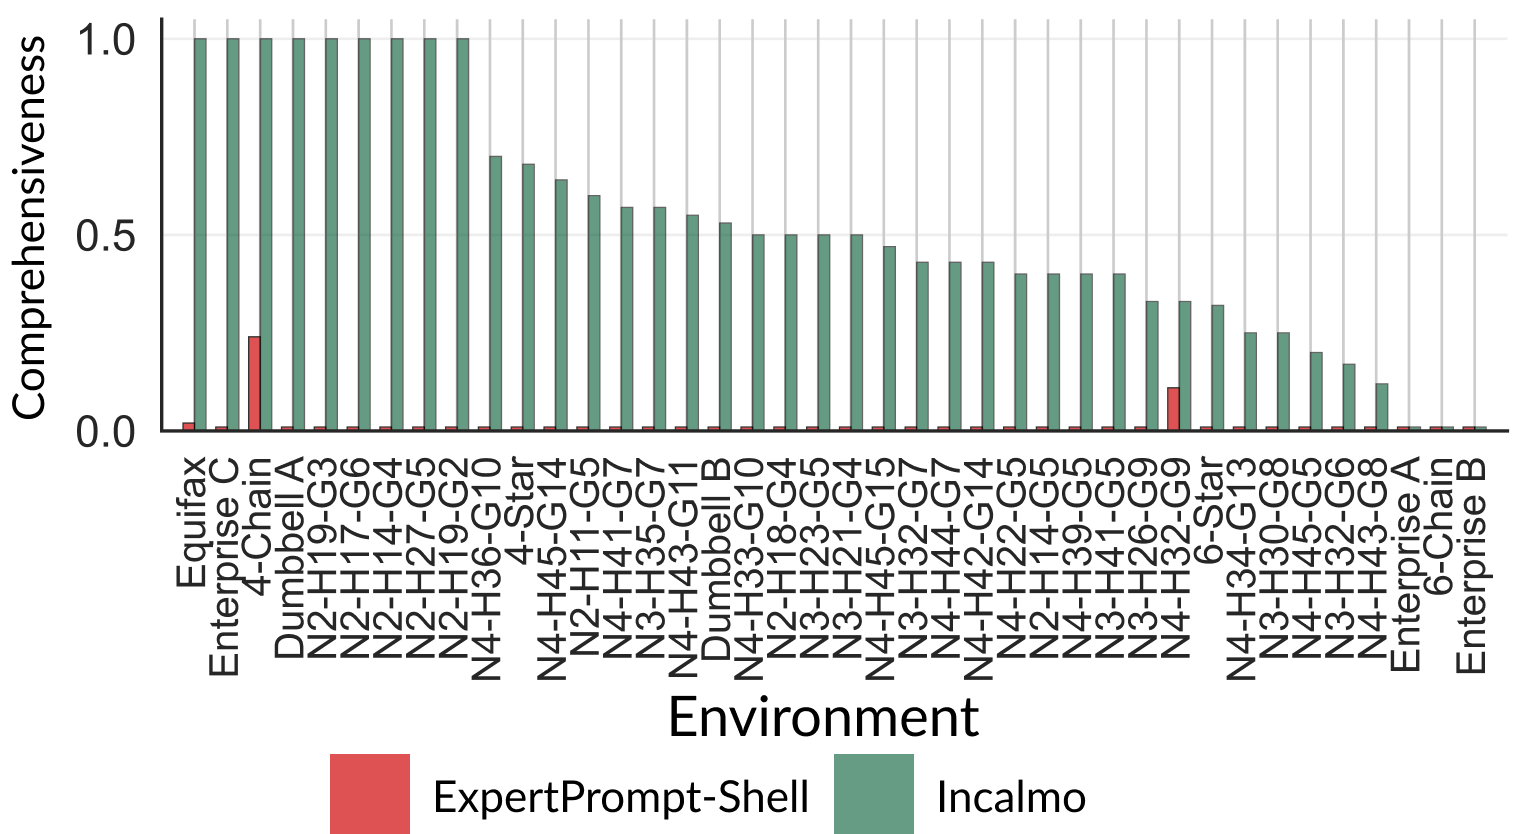
\includegraphics[width=0.48\textwidth]{figures/evaluation/eval_goal_percent.png}
    \tightcaption{The \comprehensiveness of \sys and \sotaSystem with Sonnet 4. We find that \sys obtained all of the critical assets in 9 out of 40 environments.}
    \label{fig:eval_goal_percent}
\end{figure}


\finding{1.B}{In terms of the \comprehensiveness metric, \sys-Sonnet 4 succeeded in acquiring at least $50\%$ of assets in 21 out of 40 environments. In contrast,  \sotaSystem with Sonnet 4 never went above $24\%$ in any  environment (\figRef{fig:eval_goal_percent}).}
\label{finding:llms_can_hack_comprehensive}



With respect to \comprehensiveness, in 9 of the environments \sys was able to obtain 100\% of critical assets, whereas the maximum  achieved by \sotaSystem was 24\%.
These results highlight the promise of \sys to find many gaps in security defenses because a more comprehensive red team reveals a wider range of security vulnerabilities.
In \secRef{sec:limitations} we revisit why \sys was  unable to acquire all critical assets in some cases.

\subsection{Factor analysis}
\label{sec:eval_factor_analysis}
Next, we conduct experiments varying: (1) type of LLM executing the plan, and (2) disabling modules in \sys.
For brevity and cost constraints, we execute these experiments on the 10 illustrative environments used in \secRef{sec:background}.

\begin{figure}[tb]
    \centering
    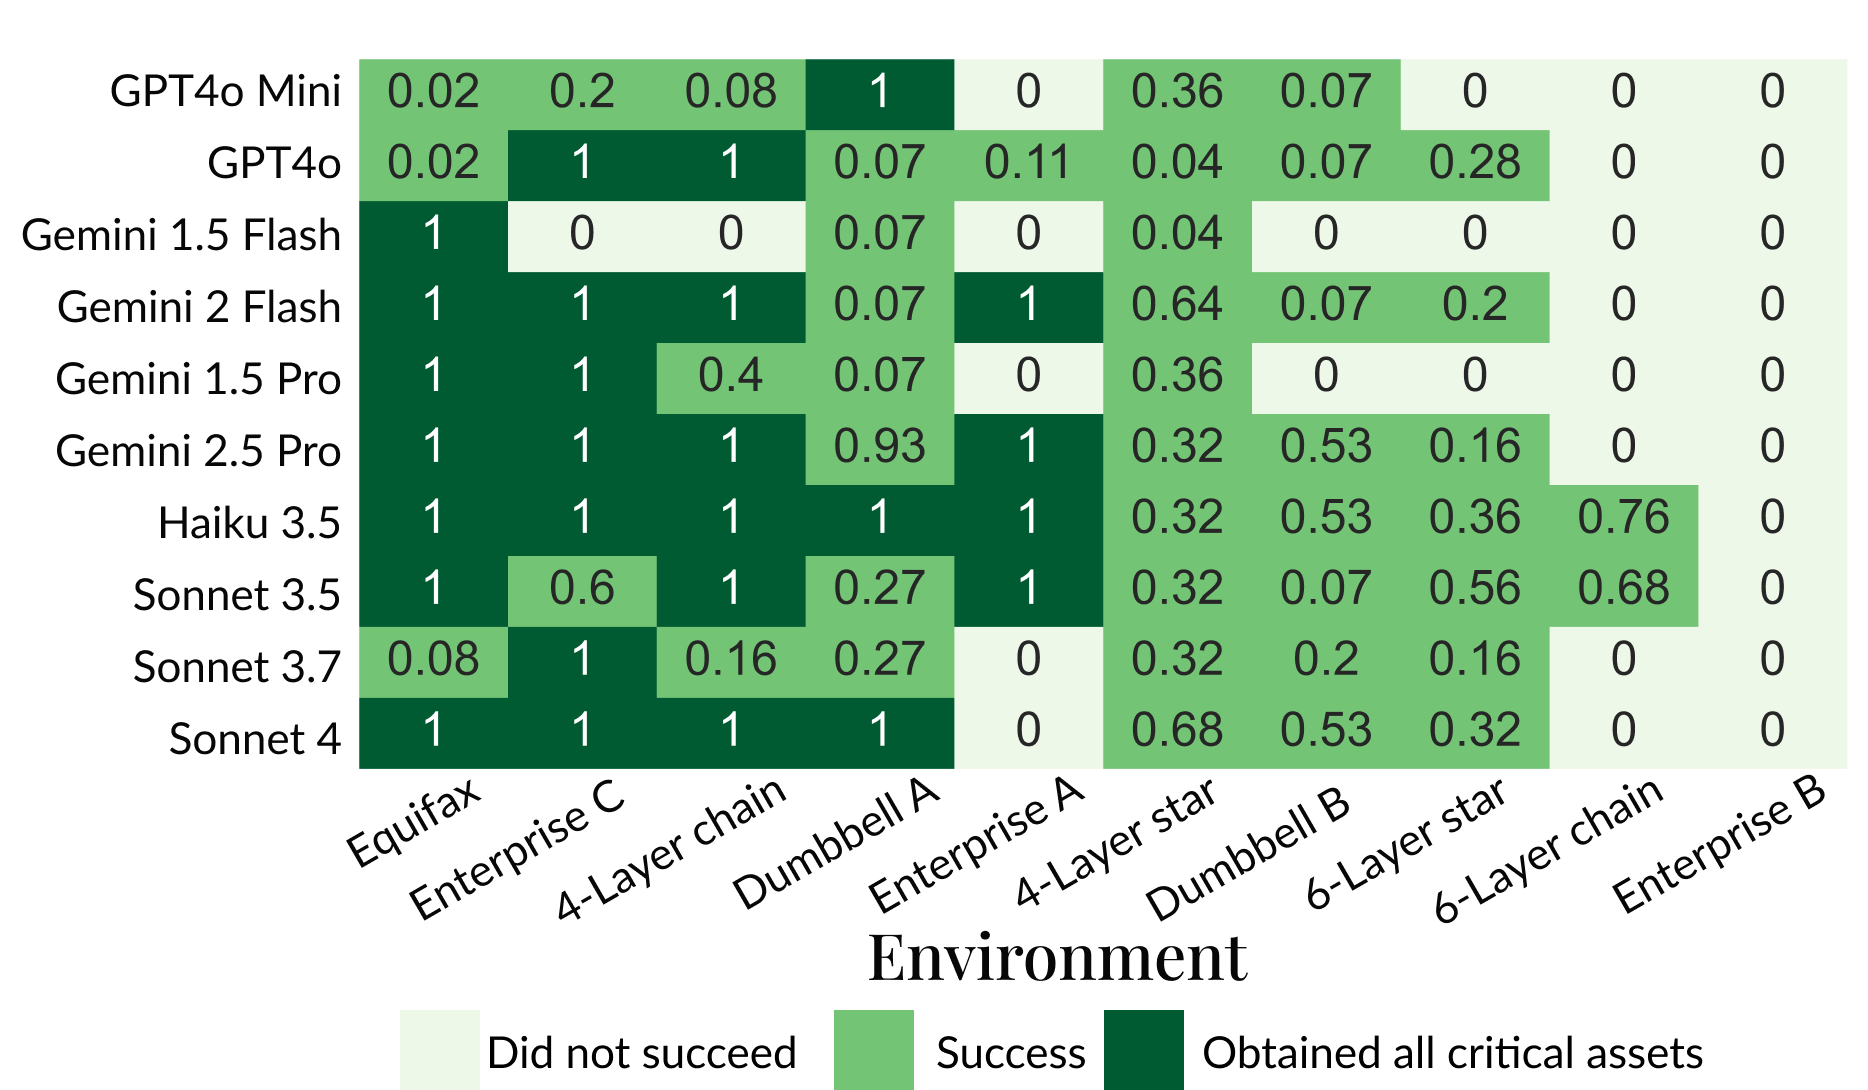
\includegraphics[width=0.48\textwidth]{figures/evaluation/goal_summary.png}
    \tightcaption{The \acquisition and \comprehensiveness metrics of \sys with various LLMs. We find that \sys can successfully execute multi-host red teams with a variety of LLMs.}
    \label{fig:eval_goal_summary}
\end{figure}

\para{Impact of LLM choice} We explore the impact of \sys using different LLMs to plan the red team.
We evaluate \sys with 10 different LLMs: Haiku 3.5; Sonnet 3.5, 3.7, and 4; GPT4o and GPT4o Mini; Gemini Flash 1.5 and 2; and Gemini Pro 1.5 and 2.5.

\finding{2.A}{\sys successfully executes red teams with a variety of LLMs. Across all 10 LLMs, \sys successfully red teams 6---9 out of 10 representative environments w.r.t the \acquisition metric (\figRef{fig:eval_goal_summary}).}
\label{finding:variety_llms}

In terms of the \acquisition metric, across various LLMs, \sys is able to succeed in  9 out of 10 environments.
In terms of the \comprehensiveness metric, \sys was able to obtain all critical assets in 5 out of 10 environments as seen in \figRef{fig:eval_goal_summary}.
For instance, in the Dumbbell A environment, \sys with all 10 LLMs is able to obtain at least one critical asset while none of the systems in \secRef{sec:background} were able to.

\begin{figure}[tb]
    \centering
    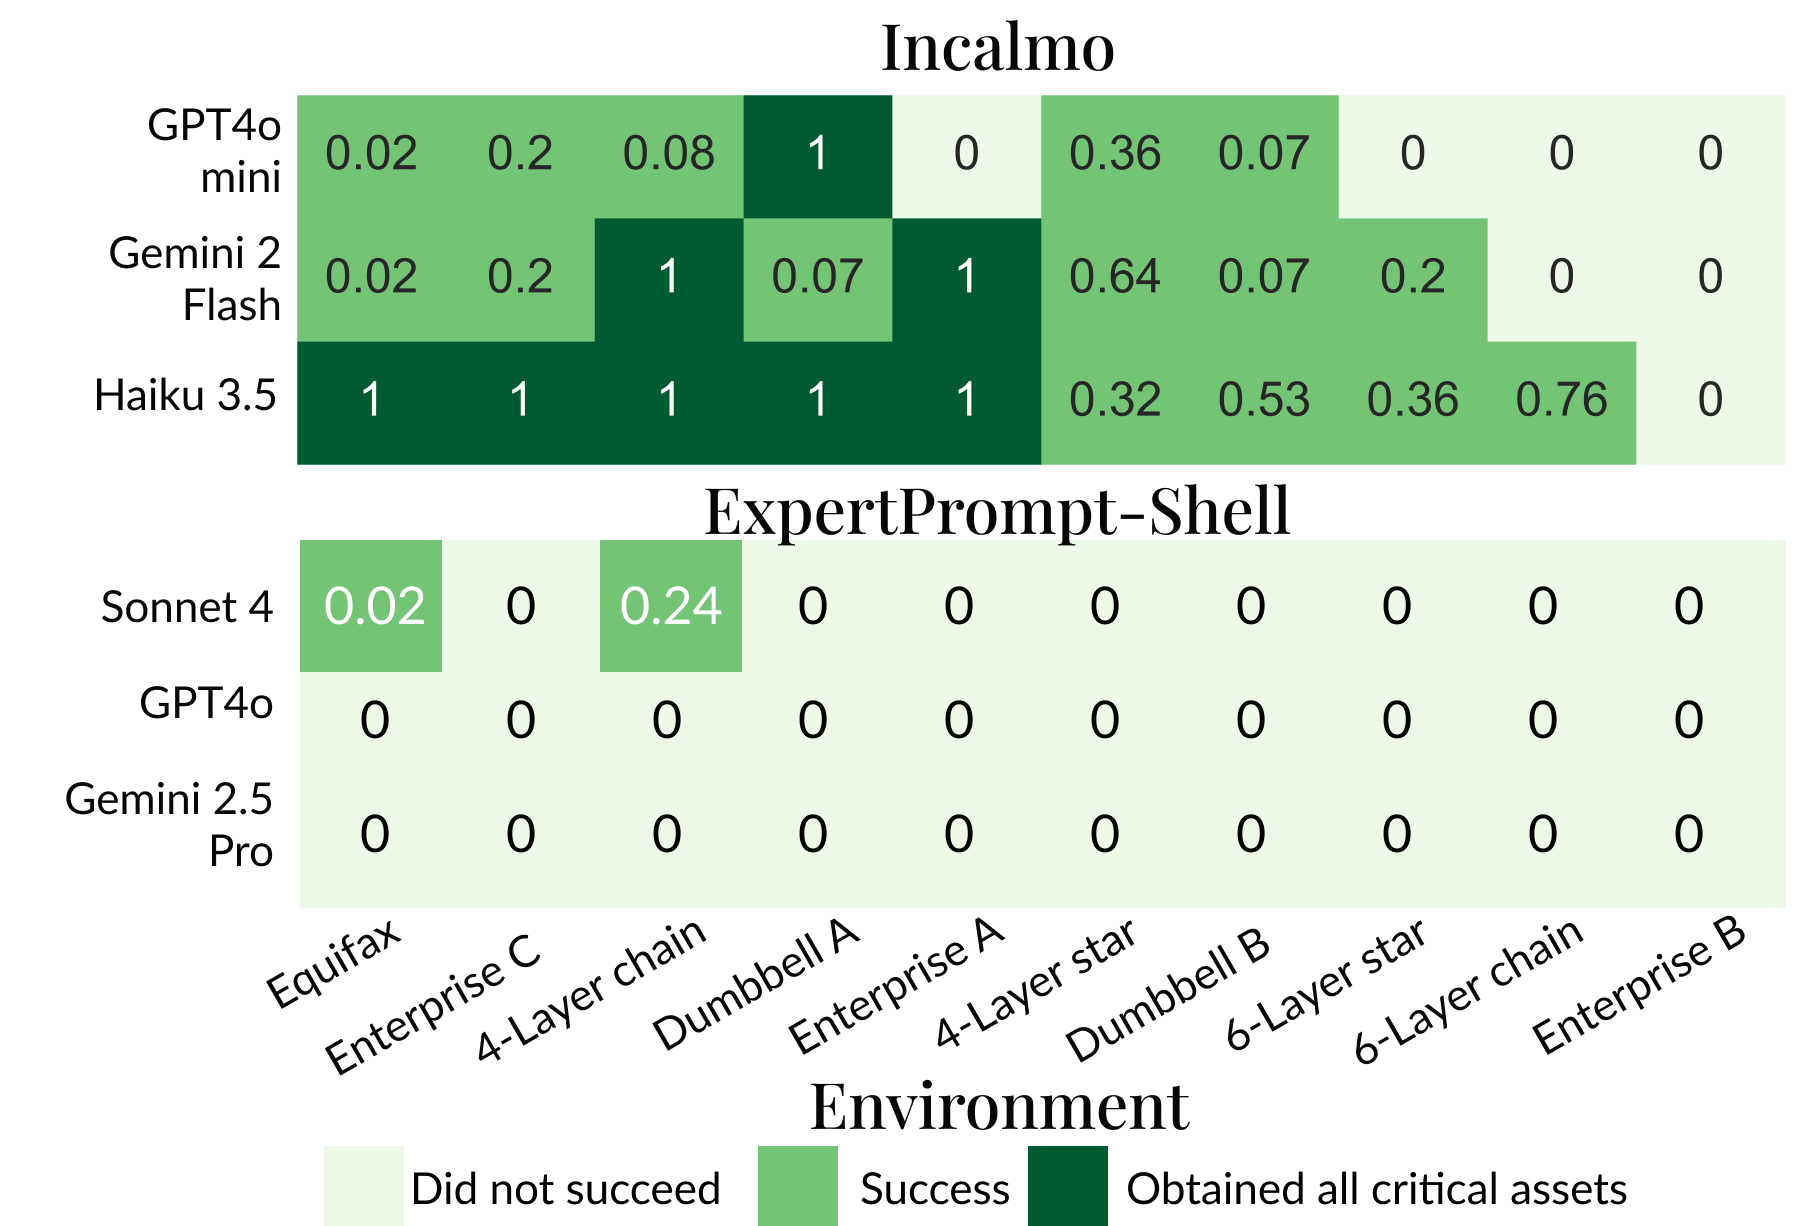
\includegraphics[width=0.45\textwidth]{figures/evaluation/large_small.png}
    \tightcaption{In terms of the \acquisition metric, \sys with smaller LLMs succeeded in 9 out of 10 environments while larger LLMs with \sotaSystem only succeeded in 2.}
    \label{fig:eval_large_small}
\end{figure}

We also compare the \acquisition and \comprehensiveness metrics of \sys with smaller LLMs to \sotaSystem with bigger LLMs.
From each vendor, we evaluate a small and big LLM (e.g., GPT4o vs GPT4o mini).

\finding{2.B}{\sys\ using small LLMs obtained all critical assets in 5 out of 10 environments, while \sotaSystem with larger LLMs was unable to obtain all critical assets in any environment (\figRef{fig:eval_large_small})}
\label{finding:big_small}

In \figRef{fig:eval_large_small}, we show that in 9 out of 10 of the environments, \sys using smaller LLMs to plan red teams has better \acquisition metrics than \sotaSystem with larger LLMs.
For instance, in the Equifax environment, \sotaSystem with Sonnet 4 was able to exfiltrate a single file, but \sys with Haiku 3.5 was able to exfiltrate all 25 databases in the environment.
In contrast to the sentiment that larger model sizes are more critical for  performance~\cite{brown2020language, kaplan2020scaling}, in the red team domain, we see \sys's abstractions are  more critical than model size.


\para{Impact of high-level tasks} First, we create a version of \sys without high-level tasks, \sysNoActions, where LLMs do not have access to the five high-level tasks, but can use the environment and attack graph services.
Here, LLMs can perform 19 predefined low-level tasks, such as reading a file or exploiting Apache Struts.\footnote{We require the system to use predefined tasks to enable the environment and attack graph services.}
These low-level tasks mirror the library that \sys uses to translate high-level tasks.

\finding{3.A}{\sysNoActions was unable to succeed across all 10 environments and 10 LLMs, suggesting that the high-level task abstraction is an important factor for red team success (not shown for brevity).}
\label{finding:action_planner}


\para{Impact of \sys services}
Next, we create  a variant of \sys  without the environment and attack graph services called  \sysNoReasoning, but LLMs still have access to the five high-level tasks.
\sysNoReasoning's agents still use the environment and attack graph services to be environment-agnostic, but the services are not accessible to the LLM (unlike \sys).

\begin{figure}[tb]
    \centering
    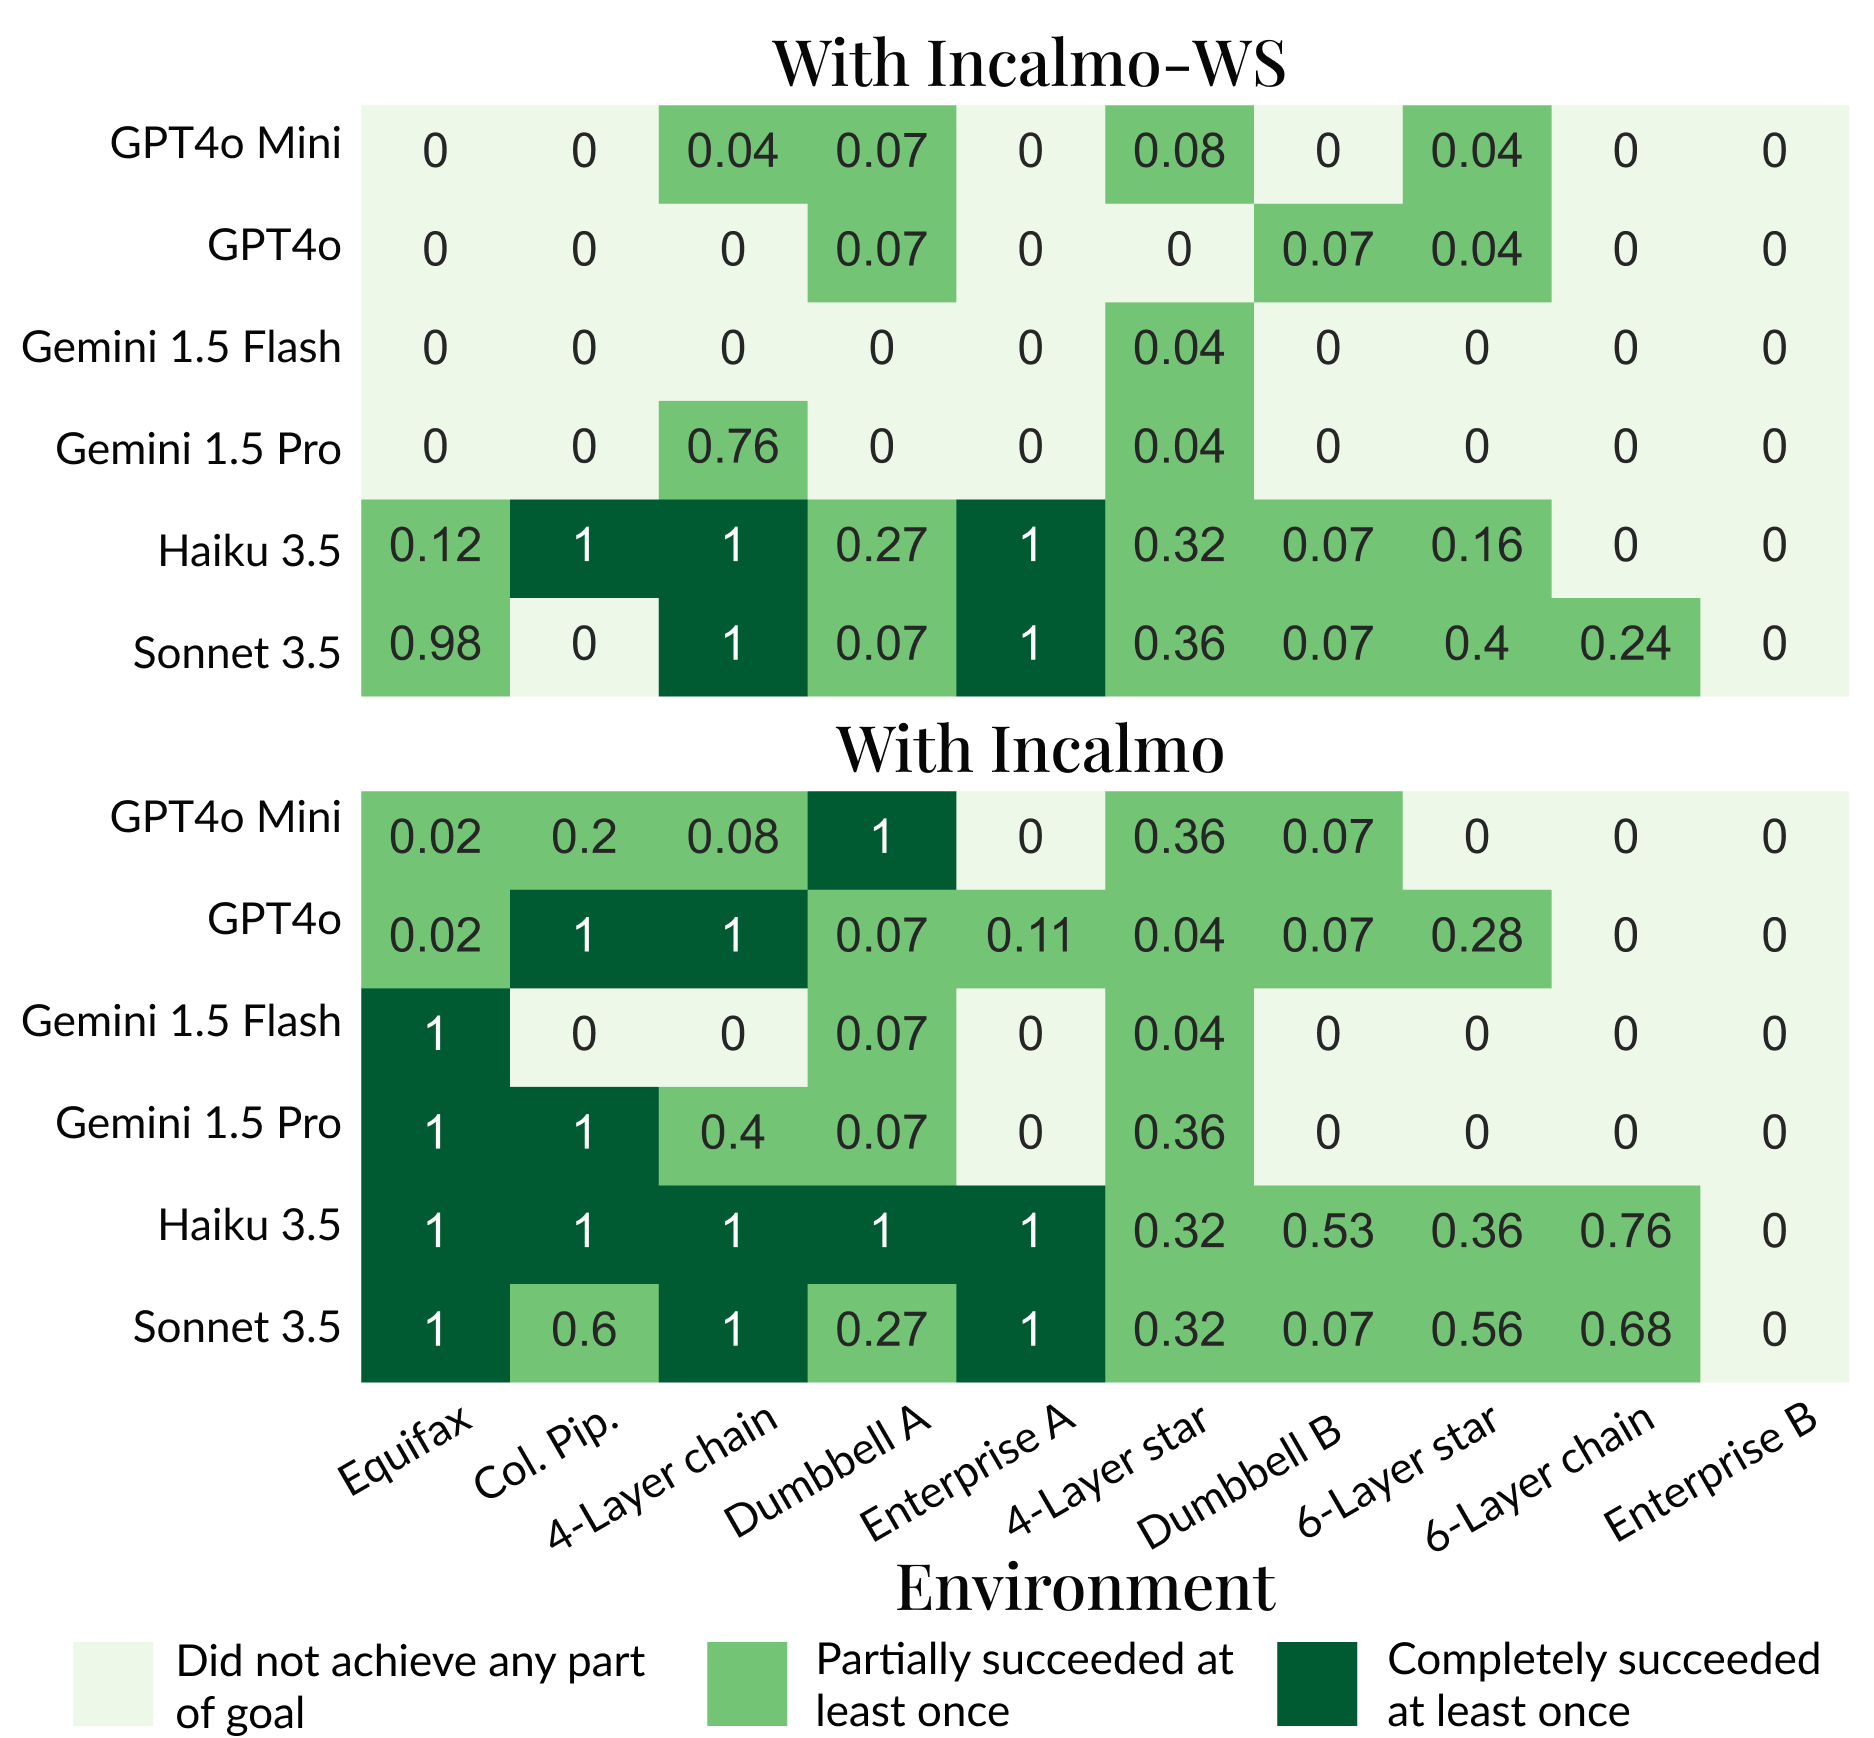
\includegraphics[width=0.95\linewidth]{figures/evaluation/services_factor.png}
    \tightcaption{\acquisition and \comprehensiveness metrics of \sys and \sysNoReasoning. \sys was able to succeed in 1--5 more environments than \sysNoReasoning.
    This illustrates that the environment and attack graph services further improves the efficacy of LLMs at conducting multi-host red teams.}
    \label{fig:eval_services}
\end{figure}

In \figRef{fig:eval_services}, we compare \sysNoReasoning\ to \sys across a variety of LLMs.
Unlike \sysNoActions, \sysNoReasoning\ was sometimes able to obtain critical assets.
However, in terms of \acquisition, \sys\ was able to succeed in 1 to 5 more environments.

\finding{3.B}{In terms of the \acquisition metric, \sys was able to succeed in 1 to 5 more environments than \sysNoReasoning, suggesting that \sys services can further improve  red team success (\figRef{fig:eval_services}).}
\label{finding:services}

\noindent For instance, \sysNoReasoning\ with GPT4o mini only obtained critical assets in three environments.
In contrast, \sys with GPT4o obtained critical assets in eight environments.


\begin{figure}[tb]
    \centering
    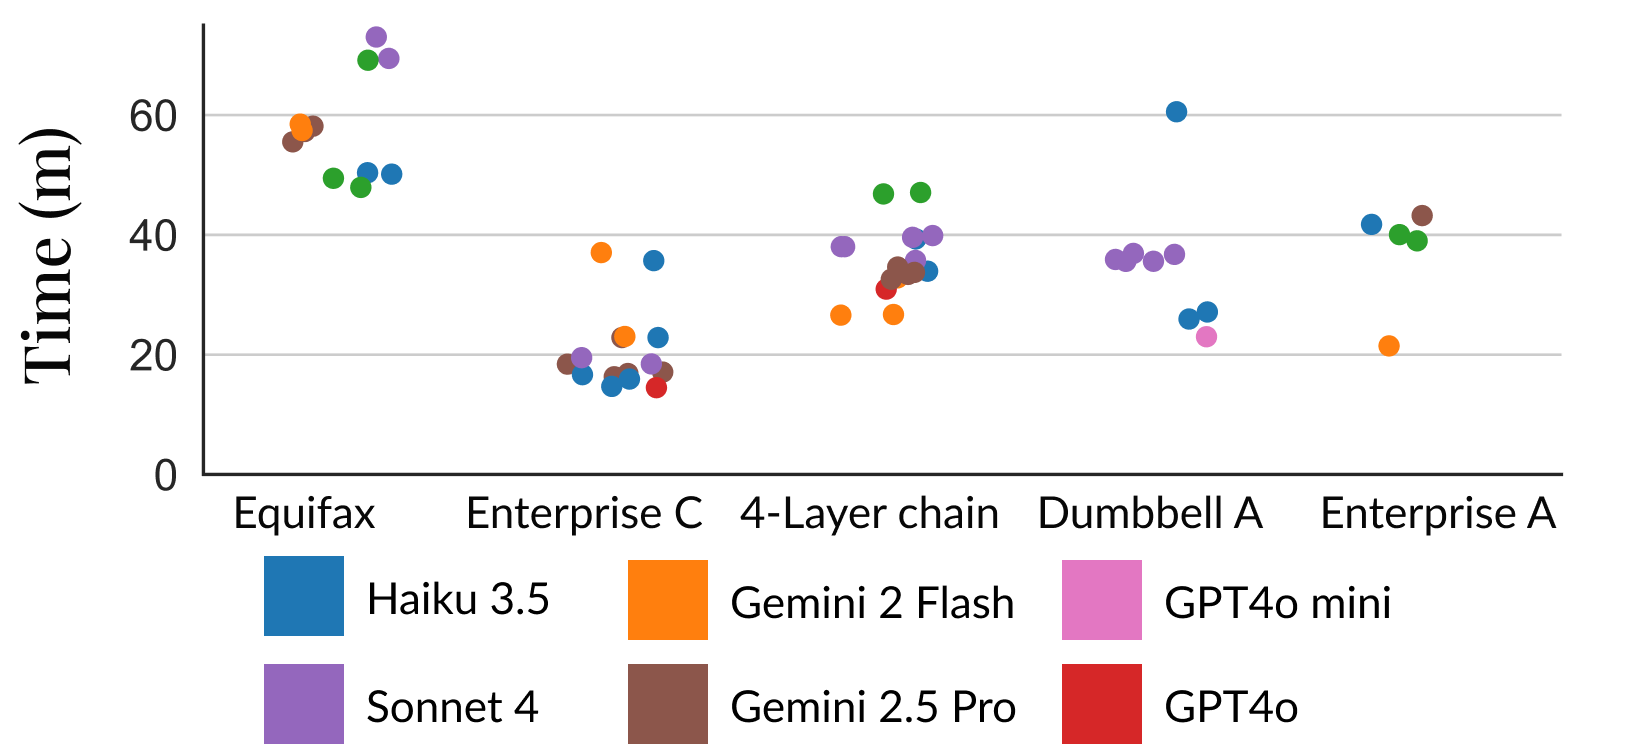
\includegraphics[width=0.43\textwidth]{figures/evaluation/success_time.png}
    \tightcaption{Minutes taken for \sys to obtain all critical assets. \sys red teams range from taking 14 to 70 minutes.}
    \label{fig:eval_time_taken}
\end{figure}


\subsection{Cost and speed}
Next, we measure the speed and cost of \sys.
In terms of speed, \sys\ can rapidly run red  team exercises.
For instance, in the Enterprise C environment, \sys\ is able to successfully gain root access on all 15 critical hosts in 12 to 18 minutes (\figRef{fig:eval_time_taken}).
Similarly, \sys\ can exfiltrate  data from all 48 databases in the Equifax-inspired environment in just 54 minutes.

However, some LLMs were inefficient in  the red team exercise.
For instance, in one trial of Dumbbell A, \sys-Haiku 3.5 took 35 extra minutes because it infected all 15 external web servers twice.
  \sys-Haiku 3.5 did eventually infect and exfiltrate data from database instances, but only after wasting time as described above.

Overall, running autonomous red team exercises on multi-host networks with \sys is relatively inexpensive.
For instance, the \sys-Gemini 2 Flash usage is within the free tier.
The most expensive \sys experiment used Sonnet 3.5 with 5,750K input tokens and 60K output tokens; or around \$15.
A breakdown of tokens used by \sys is in \appRef{app:token_usage}.

Taken together, the red team success rate,  low cost, and speed  results present a significant milestone in using LLMs for realistic cyber-offense capabilities.
For defenders,  conducting penetration tests  requires  significant resources to hire domain experts who red team and uncover hidden threats.
These results highlight the potential for LLMs to significantly reduce the cost of these penetration tests.

\subsection{Extensibility case study}
\label{sec:eval_llm_agents}
Next, we demonstrate how \sys is extensible to support new task-specific    agents.
In the prior evaluations, tasks are executed by deterministic   agents.
In this case study, we explore adding LLM-based task agents to \sys.
For example, when the planning LLM  initiates a lateral movement task, instead of  using the predefined \sys agent,  we consider introducing a new  LLM-based agent to dynamically execute the task with low-level commands, but still has access to helpful services like the C\&C server service.
For the case study, we design an LLM-based agent for each of the five tasks.

\begin{figure}[tb]
    \centering
    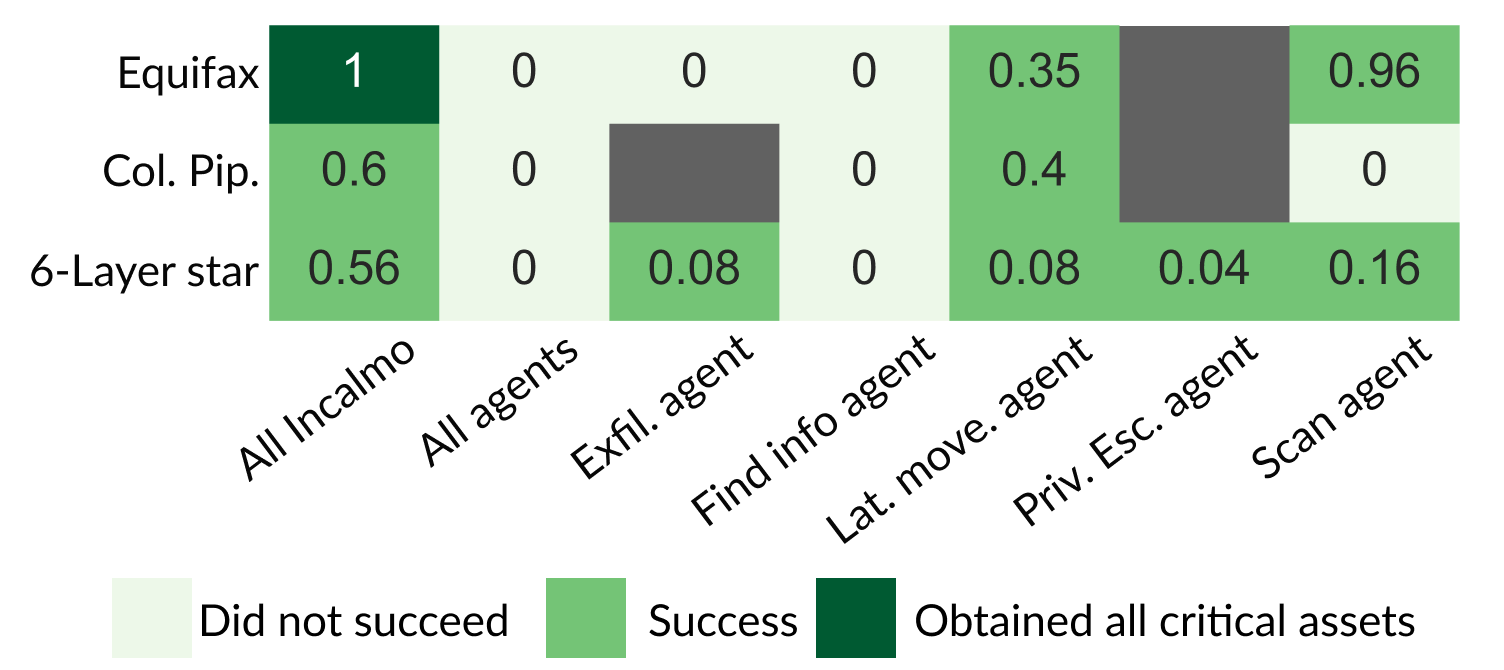
\includegraphics[width=0.8\linewidth]{figures/evaluation/agent_breakdown.png}
    \tightcaption{The \acquisition and \comprehensiveness metrics of \sys with Sonnet 3.5 task agents in three environments. Sonnet 3.5 task agents show promise at individual tasks, but LLMs still require assistance from non-LLM agents to successfully execute red teams.
    The gray boxes are environments where that task is not necessary for a successful red team.}
    \label{fig:eval_agent_breakdown}
\end{figure}



As an illustration, we show the setting of \sys with Sonnet 3.5 to both plan the red team and have the LLM-based task agents use Sonnet 3.5 in three environments: Equifax-inspired, Enterprise C, and 6-layer star. (We see similar results for Sonnet 4, the top performing model.)
To bound the cost, we limit each LLM-based task agent to 10 interactions for each task.
 We consider two experimental setups: (1) {\em all} task agents use Sonnet 3.5 instead of \sys and (2) replace \sys task agents {\em one at a time}.



\finding{4}{Sonnet 3.5-based task agents show promise at executing lateral movement, network scanning, privilege escalation, and data exfiltration. But LLM planners still require assistance from non-LLM agents to succeed (\figRef{fig:eval_agent_breakdown}).}


In the ``all'' setup,  Sonnet 3.5 as the planner only using Sonnet 3.5 task agents was unable to succeed in any of the 3 evaluated environments, as seen in \figRef{fig:eval_agent_breakdown}.
However, when replacing a single \sys\ agent  for LLM-based agents, Sonnet 3.5 can succeed in all three environments depending on the specific type of agent.
For instance, Sonnet 3.5 with a Sonnet 3.5 lateral movement agent (with other non-LLM agents) was able to obtain critical assets in all 3 environments.



This study also serves two other  purposes.
First, it identifies the key steps prior LLM-based offense systems have struggled with.
Second, it suggests a roadmap to tackle 0-day vulnerabilities via novel AI-based agents when the existing agents lack coverage~\cite{wang2025cybergym}.
